%!TEX root = ../main.tex

\section{lwIP}
lwIP (lightweight IP) (\cite{lwip_docs}, \cite{lwip_wiki}) is an open-source implementation of the TCP/IP stack for embedded systems. Specifically, it implements the Ethernet, ARP, IP, TCP, and UDP protocols. It allows the implementation of user applications with networking requirements on embedded systems.

The most fundamental data structure of lwIP is the p\_buf (packet buffer). p\_buf is used for organizing packets and storing them in memory and is used in all layers of the stack. It contains the headers and data of the packet and additional information such as its size. Along with the p\_buf structure, functions for its processing are provided, such as creation, deletion, extension, etc.

The datapath followed by an incoming packet starts with its reception. Here, the processor is notified through an Ethernet Controller interrupt for the arrival of the new packet. When the processor becomes available, it retrieves the packet from the incoming queue of the Ethernet Controller and creates a new p\_buf for it. Next, the p\_buf is passed upwards from layer to layer. Each layer performs the appropriate processes on the packet, removes its header, and passes it to the next layer. If any layer decides that the packet should be dropped due to failing necessary checks or when it reaches the last processing layer, the p\_buf is deleted an memory is reclaimed. Outgoing packets follow the reverse path.

Each layer offers an interface to other layers. This interface essentially consists of the actions of receiving and transmitting a packet, and some additional layer-specific function. For example, the interface of the IP layer is shown in Listing \ref{lst:ip_interface}.\\

\noindent
\begin{minipage}{\linewidth}
\begin{lstlisting}[style=mycodestyle, label={lst:ip_interface}, caption={IP layer's interface in lwIP}]
struct netif * ip_route(struct ip_addr *dest);

err_t ip_input(struct pbuf *p, struct netif *inp);

err_t ip_output(struct pbuf *p, struct ip_addr *src, struct ip_addr *dest, u8_t ttl, u8_t tos, u8_t proto);

err_t ip_output_if(struct pbuf *p, struct ip_addr *src, struct ip_addr *dest, u8_t ttl, u8_t tos, u8_t proto, struct netif *netif);
\end{lstlisting}
\end{minipage}\\

As observed, the interface consists of input and output functions, and a specialized function of the IP protocol used for routing (ip\_route).
Lastly, each protocol has multiple parameters that can be configured by the designer, such as the TCP timeout, the maximum packet size, etc.

\section{IPsec}
The IPsec implementation is integrated into the existing codebase of lwIP, as mentioned in Chapter ~\ref{ch:4.2.2}. The software development is divided into two parts. The first involves creating in isolation a software library that provides IPsec functionality, and the second involves interfacing and integrating this library with lwIP. The components of the library and their relationships are illustrated in Figure \ref{fig:figure_6.1}. Below, the individual components of the library created for the various IPsec functions and the method of integration with lwIP are explained.


% fig 6.1
\begin{figure}
\centering
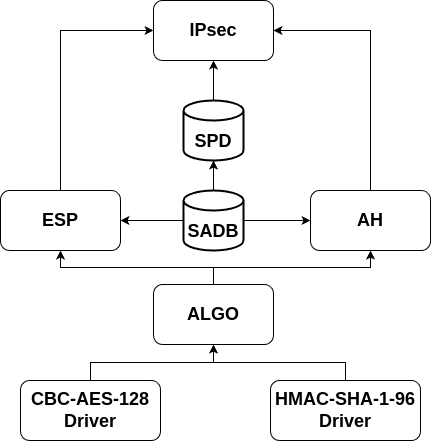
\includegraphics[width= 0.6\textwidth]{figure_6.1}\\
\caption{  Software architecture diagram for the custom IPsec library }
\label{fig:figure_6.1}
\end{figure}

\subsection{IPsec}
The library implementing IPsec provides two functions, one for processing inbound traffic and one for processing outbound traffic. The inbound function is called by the ip\_input of the IP after the packet has been processed by the IP. The outbound function is called at the beginning of the ip\_output\_if  so that every outgoing packet is first processed by IPsec before proceeding. ipsec\_output returns a code to ip\_output\_if so that the latter can select the operations to perform. The function signatures are shown in Listing \ref{lst:ipsec_interface}.\\

\noindent
\begin{minipage}{\linewidth}
\begin{lstlisting}[style=mycodestyle, label={lst:ipsec_interface}, caption={IPsec implemented interface}]
void ipsec_input(struct pbuf *p, struct netif *inp);

u8_t ipsec_output(struct pbuf *p, struct pbuf **p_new, struct ip_addr *src, struct ip_addr *dest, u8_t ttl, u8_t tos, u8_t proto, struct netif *netif);
\end{lstlisting}
\end{minipage}\\

The input function takes the $pbuf$ of the incoming packet and the Ethernet interface where the arrival occurred. Firstly, it extracts the packet fields' values and issues a SADB lookup. If the packet is not matched with any SA, it is discarded. If there is a match, depending on the protocol referenced in the SA, either esp\_input or ah\_input is called. After these functions finish processing the packet and no conditions for packet rejection arise, the SPD is checked to ensure that the packet complies with the policy. If the packet passes the SPD check, it is forwarded to ip\_input as a pure IP packet to continue its path in the TCP/IP stack.

The output function takes the pbuf of the outgoing packet, a pbuf to which the processed packet will be assigned as a result of ipsec\_output, the IP addresses of the sender and receiver, the TTL and TOS values of the packet, and the Ethernet interface that will perform the transmission. The function returns a code, whose values correspond to:

\begin{outline}
\1 RET\_IPSEC\_ERROR if an errors occur,
\1 RET\_IPSEC\_BYPASS for applying the BYPASS policy,
\1 RET\_IPSEC\_APPLY for applying the PROTECT policy,
\1 RET\_IPSEC\_DISCARD for applying the DISCARD policy.
\end{outline}

The ipsec\_output initially searches the SPD. If no policy is found, the packet is discarded. If found, if it's a DISCARD policy, the function simply returns the RET\_IPSEC\_DISCARD code. If it's BYPASS traffic, no processing is performed on the packet, and the function returns with the RET\_IPSEC\_BYPASS code. If it's PROTECT traffic, depending on the protocol defined in the policy's SA, the packet is passed to either ah\_output or esp\_output. If they return without errors, the function returns with the RET\_IPSEC\_APPLY code; otherwise, with the RET\_IPSEC\_ERROR code. If an error occurs at any point in ipsec\_output, it returns with the RET\_IPSEC\_ERROR code.

The ipsec\_output returns to ip\_output\_if, which has been modified to interpret the return value of ipsec\_output properly. Thus, when RET\_IPSEC\_ERROR is returned, it discards the packet and reports an error. When RET\_IPSEC\_BYPASS is returned, the regular IP processing is executed. If RET\_IPSEC\_APPLY is returned, the packet is a ready IP packet for transmission due to processing by ah\_output or esp\_output and is sent without further processing. Finally, if RET\_IPSEC\_DISCARD is returned, ip\_output\_if discards the packet and releases the memory.



\subsection{AH and ESP}
The main processing of packets in IPsec is performed by the AH and ESP protocols. These protocols add additional headers and populate the header fields. Packets undergo cryptographic transformations for outgoing traffic, while header fields are checked and packets undergo reverse cryptographic transformations and checks for incoming traffic.

For incoming traffic, the implementation of AH and ESP provide an input function, ah\_input and esp\_input respectively. These functions are called by ipsec\_input, with arguments being the pbuf of the packet and the corresponding SA. Both functions start by checking the Sequence Number. Then the authentication and integrity checks follow which are mandatory for AH but optional for ESP. Next, for ESP only, the packet gets decrypted. The parameters for all these operations are found in the applicable SA. Finally, both functions consult the SA regarding the IPsec mode in which they should process the packet. In the case of Transport Mode, the IPsec header is removed, and the IP header is prepended to the payload. For Tunnel Mode, the outer header and the IPsec header are removed, leaving the inner header intact. A the end of these processes, we obtain an IP packet which is forwarded to ip\_input accordingly. The interfaces for AH and ESP inbound process are shown in Listing \ref{lst:ah_esp_in_interface}.\\

\noindent
\begin{minipage}{\linewidth}
\begin{lstlisting}[style=mycodestyle, label={lst:ah_esp_in_interface}, caption={AH and ESP inbound processing  interfaces}]
int ah_input(struct pbuf* p, struct sa_entry* sa);
int esp_input(struct pbuf* p, struct sa_entry* sa);
\end{lstlisting}
\end{minipage}

For outbound traffic, the functions ah\_output and esp\_output are provided, which are called by ipsec\_output. Their arguments include the pbuf of the packet, a new pbuf where the processed packet will be placed, the policy entry found by ipsec\_output, as well as the IP addresses of the sender and recipient, the values of TTL and TOS, and the interface from which the packet will be sent. TTL and TOS are provided by the Transport Layer protocols and are given to ah\_output and esp\_output so that they can construct the inner IP header and, if it is tunnel mode traffic, the outer IP header too. The interfaces for AH and ESP inbound process are shown in Listing \ref{lst:ah_esp_out_interface}.\\

\noindent
\begin{minipage}[t]{\linewidth}
\begin{lstlisting}[style=mycodestyle, label={lst:ah_esp_out_interface}, caption={AH and ESP outbound  processing interfaces}]
err_t ah_output(struct pbuf *p, struct pbuf **p_new, struct spd_entry* spdentry, struct ip_addr *src, struct ip_addr *dest, u8_t ttl, u8_t tos, u8_t proto, struct netif *netif);

err_t esp_output(struct pbuf *p, struct pbuf **p_new, struct spd_entry* spdentry, struct ip_addr *src, struct ip_addr *dest, u8_t ttl, u8_t tos, u8_t proto, struct netif *netif);
\end{lstlisting}
\end{minipage}

Packet processing begins with the placement of the inner IP header if in Tunnel Mode. Then, for ah\_output, the AH header is placed, followed by the outer IP header, and finally, the packet goes through the integrity and authentication algorithm, and the ICV value is placed in the appropriate field before being handed back to ipsec\_output.

In esp\_output, after the possible placement of the inner IP header, padding and IV are added, followed by encrypting all of the above together with the payload. Then, the ESP header is added, and if integrity is used, the integrity algorithm is applied. The ICV of the integrity algorithm is placed at the end of the packet, and finally, the outer IP header is added. Upon returning from esp\_output to ipsec\_output, the processed packet is ready to continue its transmission.


\subsection{SADB and SPD}
The SADB is implemented as a unidirectional linked list. Each entry in the SADB represents an SA. The structure implemented to represent an SA contains:

\begin{outline}
\1 the SPI number
\1 the IANA number of the protocol
\1 the mode corresponding to the traffic (transport or tunnel)
\1 the packet sequence number (Sequence Number)
\1 The authentication algorithm used by AH (if applicable, i.e., if AH protocol \1 is used for this traffic)
\1 If applicable, the key is also retained.
\1 The authentication algorithm used by ESP (if applicable, i.e., if ESP \1 protocol is used and authentication is used for this traffic simultaneously)
\1 If applicable, the key is also retained.
\1 The encryption algorithm of ESP (mandatory if ESP is used).
\1 If applicable, the key is also retained.
\1 A pointer to the next SADB entry to maintain a unidirectional linked list.
\end{outline}

\noindent
The definition of the structure is shown in Listing \ref{lst:sadb}.\\

\noindent
\begin{minipage}{\linewidth}
\begin{lstlisting}[style=mycodestyle, label={lst:sadb}, caption={The SADB entry structure}]
struct sa_entry
{
	u32_t spi;
	u8_t protocol;	
	u8_t mode;		// Transport or Tunnel
	
	/* Current Connection */
	u32_t seqnum; 
	
	/* Algorithms */
	struct auth_algo* ah_auth_algo;
	u8_t* ah_auth_key;
	
	struct enc_algo* esp_enc_algo;
	u8_t* esp_enc_key;
	
	struct auth_algo* esp_integrity_algo;
	u8_t* esp_integrity_key;
	
	/* Linked entries*/
	struct sa_entry *next;

}__attribute__((packed));
\end{lstlisting}
\end{minipage}\\

The structures auth\_algo and enc\_algo are created to add a flexible interface for cryptographic algorithm integration. They serve as an intermediate layer between IPsec and the algorithm interfaces. If a new cryptographic algorithm needs to be used, it is sufficient to create an auth\_algo or enc\_algo structure (depending on the type of algorithm) so that it can be directly utilized by the specific IPsec implementation.

The SADB library provides functions for creating and adding a new SA to the database and for searching for an SA based on the SPI and protocol number values. The search function returns the entry if found. The signatures of these functions are shown in Listing \ref{lst:sadb_interface}.\\

\noindent
\begin{minipage}{\linewidth}
\begin{lstlisting}[style=mycodestyle, label={lst:sadb_interface}, caption={The SADB interface}]
struct sa_entry *sa_lookup(u32_t spi, u8_t proto);

struct sa_entry* sa_add(u32_t spi, u8_t protocol, u8_t mode, 
				  struct auth_algo* ah_auth_algo, u8_t* ah_auth_key,
				  struct enc_algo* esp_enc_algo, u8_t* esp_enc_key,
				  struct auth_algo* esp_integrity_algo, u8_t* esp_integrity_key);
\end{lstlisting}
\end{minipage}\\

Similarly to SADB, SPD is implemented as a unidirectional linked list. Each entry in the list represents a policy and includes:
\begin{outline}
    \1 The sender's IP address
    \1 The sender's subnet mask
    \1 The receiver's IP address
    \1 The receiver's subnet mask
    \1 The protocol's IANA number
    \1 The type of policy (PROTECT, BYPASS, DISCARD)
    \1 The direction of traffic (IN or OUT)
    \1 The IPsec protocol used in the case of the PROTECT policy (AH or ESP)
    \1 The mode (Transport or Tunnel)
    \1 The sender's IP address of the tunnel
    \1 The receiver's IP address of the tunnel
    \1 The SA that characterizes the policy's traffic
    \1 A pointer to the next entry in the SPD to implement the unidirectional linked list.
\end{outline}

\noindent
The definition of the structure is shown in Listing \ref{lst:spd_entry}.\\

\noindent
\begin{minipage}{\linewidth}
\begin{lstlisting}[style=mycodestyle, label={lst:spd_entry}, caption={The SPD entry strucutre}]
struct spd_entry{

	struct 
	ip_addr*	src ;			/**< IP source address */
	u32_t  		src_netaddr ;		/**< net mask for source address */
	struct 
	ip_addr*	dest ;			/**< IP destination address */
	u32_t		dest_netaddr ;		/**< net mask for the destination address */
	u8_t		protocol ;		/**< the transport layer protocol */
	u8_t		policy ;			/**< defines how this packet must be processed*/
	u8_t		direction;		/**< defines IN or OUT traffic direction */
	u8_t		ipsec_proto;		/**< AH or ESP processing */
	u8_t		ipsec_mode;		/**< Transport or Tunnel mode */
	struct 
	ip_addr*	tunnel_src;		/**< IP tunnel source */
	struct 
	ip_addr *	tunnel_dest;		/**< IP tunnel destination */
	
	struct
	sa_entry*	sa ;			/**< pointer to the associated SA */
	struct
	spd_entry*	next ;			/**< pointer to the next table entry*/
}
\end{lstlisting}
\end{minipage}\\

The SPD library provides functions for creating and adding a new policy to the database, as well as for searching for a policy based on the sender's and receiver's IP and subnet mask values and the protocol number. The search function returns the entry if found. The signatures of these functions is shown in Listing \ref{lst:spd_interface}.\\

\noindent
\begin{minipage}{\linewidth}
\begin{lstlisting}[style=mycodestyle, label={lst:spd_interface}, caption={The SPD interface}]
struct spd_entry* spd_lookup(struct ip_addr *src, u32_t src_netaddr, 
struct ip_addr *dest, u32_t dest_netaddr, u8_t proto);
	
void spd_add(struct ip_addr *src, struct ip_addr *dest, u8_t proto, 
    u8_t policy, u8_t direction, u8_t ipsec_proto, u8_t ipsec_mode,
    struct ip_addr *tunnel_src, struct ip_addr *tunnel_dest,
    struct sa_entry* sa);
\end{lstlisting}
\end{minipage}\\


\section{Integration with lwIP}
The software interface of the implemented IPsec library consists of two functions, one for processing incoming packets and one for processing outgoing packets.

The modifications in lwIP are made at the IP level since IPsec belongs to this layer. For inbound traffic, the packet must pass through IPsec after being processed by IP. Thus, the ip\_input function is modified to hand over control to the IPsec input routine. Specifically, ip\_input first processes the packet, and when finished, decides which protocol to pass the packet's payload to. Here, the option of IPsec for AH and ESP protocols is introduced. Figure \ref{fig:figure_6.2} illustrates the flowchart before and after modification of the inbound processing.

% fig 6.2
\begin{figure}
\centering
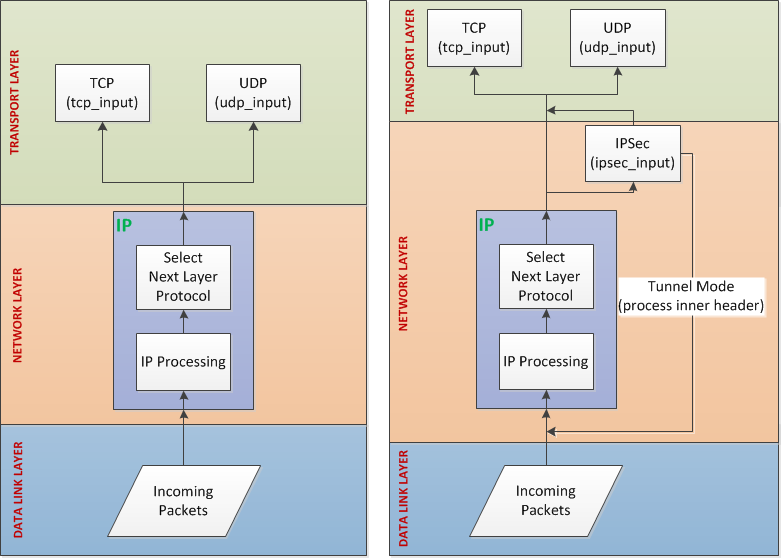
\includegraphics[width= 0.8\textwidth]{figure_6.2}\\
\caption{  Integration of inbound IPSec packet processing in lwIP }
\label{fig:figure_6.2}
\end{figure}

The function ipsec\_input serves as the interface for incoming IPsec packets. If the next hop after IP is IPsec, then the packet is handed over via ipsec\_input. At the end of IPsec processing, if the packet is in Transport Mode, it is forwarded to the appropriate Transport Layer protocol. If the packet is in Tunnel Mode, then it is passed back to the IP layer for further processing of the inner IP header and subsequently forwarded to one of the Transport Layer protocols.

For outbound traffic, the packet must first be passed to IPsec, and if it passes all the checks, it is handed over to IP for transmission. In this case, changes are made to the ip\_output\_if function. This is more heavily modified compared to ip\_input, as a considerable amount of IPsec code had to be executed before transferring the packet to the IP layer, such as searching the SPD and creating the IPsec header.

% fig 6.3
\begin{figure}
\centering
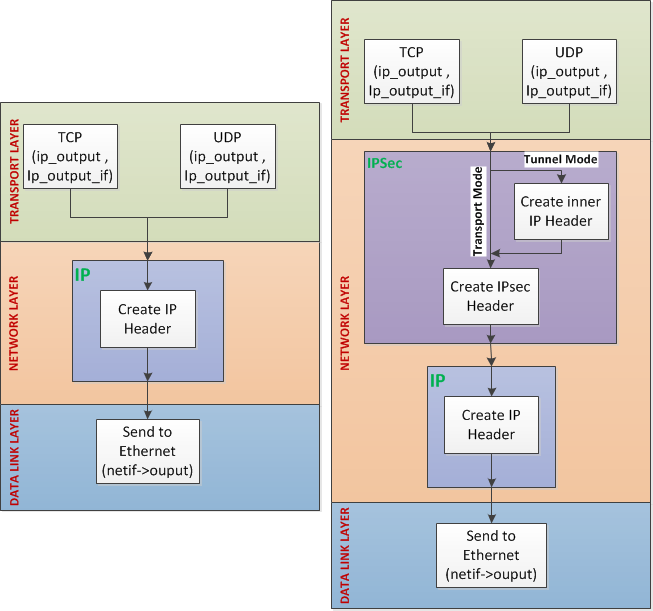
\includegraphics[width= 0.8\textwidth]{figure_6.3}\\
\caption{  Integration of outbound IPSec packet processing in lwIP }
\label{fig:figure_6.3}
\end{figure}

The flowcharts for outbound traffic of lwIP and modified lwIP are shown in Figure \ref{fig:figure_6.3}. When a packet is forwarded from one of the transport layer protocols to IP, the ip\_output or ip\_output\_if function is invoked. During execution in the modified lwIP, the packet is first processed by IPsec and then by IP. In processing by IPsec, we have two cases: the first is when the packet belongs to tunnel mode traffic, where the inner IP header is placed first, followed by the IPsec header, and the second is when we are in transport mode traffic, so only the IPsec header is placed.


\section{Software-side Interface}
Software drivers are created for the two peripherals to abstract out the details of handling the hardware interface from the rest of the software. Specifically, these drivers handle the movement of data between memory and peripherals and utilize the communication protocol of the peripheral to control its operation. They provide certain functions to the system to seamlessly execute cryptographic operations using the peripherals.

For the CBC-AES-128 peripheral, the driver has two functions, one for encrypting and one for decrypting a message. Their inputs are the memory location from which the message starts, the size of the message, the memory location from which the key starts, and the memory location from which the IV starts. Initially, the key, IV, and the first block of the message are copied from memory to the appropriate registers of the peripheral. Then, a start\_new signal is issued along with a suitable value of the EncDec signal ('0' for encryption, '1' for decryption) to notify the peripheral that a computation on a new message is starting. The driver then waits for the peripheral's ready signal to be issued. Once issued, it copies the result to the memory locations where the original block was, copies the next block, and issues a next\_block signal. It then waits again for the ready signal, then copies the result to memory, and then issues the next block. This process repeats until all input blocks are processed. It is noted here that using CBC-AES-128 with ESP relieves the driver from performing padding, as the packet already contains padding from ESP processing. The function signatures and their operation are described using pseudocode in Listing \ref{lst:aes_driver}. \\


\begin{lstlisting}[style=mycodestyle, label={lst:aes_driver}, caption={AES driver pseudocode}]
void AES128_CBC_encrypt(void* data, u32_t length,  void* key, void* iv)
{
	Copy the first 128 bits of data to the peripheral
	Copy key to the peripheral
	Copy iv to the peripheral

	Send start_new=’1’ and EncDec = ‘0’
	Wait until ready=’1’
	Copy result in the first 128 bits of data

        For all the next 128 bits blocks of data:
	   Copy the next 128 bits of data
	   Send next_block
	   Wait until ready=’1’
	   Copy result in the corresponding 128 bits of data
}

void AES128_CBC_decrypt(void* data, u32_t length, void* key, void* iv)
{
	Copy the first 128 bits of data to the peripheral
	Copy key to the peripheral
	Copy iv to the peripheral

	Send start_new=’1’ and EncDec = ‘1’
	Wait until ready=’1’
	Copy result in the first 128 bits of data

        For all the next 128 bits blocks of data:
	   Copy the next 128 bits of data
	   Send next_block
	   Wait until ready=’1’
	   Copy result in the corresponding 128 bits of data
}
\end{lstlisting}\\

For the peripheral HMAC-SHA1-96, the driver provides two functions, one for generating the MAC of a message and one for comparing a given MAC with the MAC of a message. Both functions execute the hmac-sha1-96 on the message, and their only difference is that the first one copies the MAC result to a specific memory area, while the second one compares the MAC result with another MAC and returns the comparison result. The former is used by IPsec to create the MAC of a new packet and place it in the appropriate field, while the latter is used to authenticate an incoming packet.

The procedure for handling the HMAC-SHA1-96 peripheral is as follows: initially, for each new message (packet), a reset signal is provided. Then, the driver copies the key and the first block of the message from memory to the appropriate registers of the peripheral and issues a next\_block signal. Subsequently, the driver waits for the waiting\_nxt signal to place the next block and issues the next\_block signal again. This process continues for all blocks, and once all the message blocks are processed, a msg\_done signal is issued, and the driver is then waiting for the ready signal. Finally, once the ready signal is issued, if we are in the MAC generation function, the result is copied to memory, while if we are in the comparison function, the result is compared with the given MAC, and the comparison result is returned. It is noted that the padding of the block is calculated in the driver functions and that the key size is exactly 160 bits, so no preprocessing is needed.
Below are the function signatures and their operation described using pseudocode in Listing \ref{lst:hmac_driver}.\\

\begin{lstlisting}[style=mycodestyle, label={lst:hmac_driver}, caption={HMAC driver pseudocode}]
int HMAC_SHA1_96_authenticate(void* data, u32_t datalength, void* key, 
    u32_t keylength, void* icv)
{
    Padding execution,
    Send rst
    
    For each block of 512 bits of the message:
        Copy the first 512 bits of the message
        Send next_block='1'
        Wait for waiting_nxt
        Send msg_done
        Wait for ready='1'

        If icv == result of the peripheral
            Return 1
        Else
            Return 0
}

void HMAC_SHA1_96_calculate(void* data, u32_t datalength, void* key, u32_t keylength, 
                    void* icv)
{
    Padding execution,
    Send rst
    
    For each block of 512 bits of the message:
        Copy the first 512 bits of the message
        Send next_block='1'
        Wait for waiting_nxt
        Send msg_done
        Wait for ready='1'
        Copy the result of the peripheral to icv
}

\end{lstlisting}